\section{Numerical example}
In this section we report some examples using the presented formulation to proven the good behaviour. All examples are studied in nearly incompressible limit. 

\subsection{Square problem}
First example is a unit square domain with homogeneous Dirichlet boundary conditions and we the exact solution is
\begin{equation}\label{eq:exact_solution}
u_{1} = \cos (\pi x) \sin(2\pi y), \hspace{10pt} 
u_{2} = \sin(\pi x)\cos(\pi y)\:.
\end{equation} 
%u_{1} = -2x^{2}y(1-x)^{2}(1-3y+2y^{2}), \hspace{10pt} 
%u_{2} = 2xy^{2}(1-y)^{2}(1-3x+2x^{2})\:.
The Lamé constant are fix to $\lambda = 123$ and $\mu=79.3$. %$\lambda = 123$ and $\mu=1.0$. 
By imposition of the previously exact solution one obtain for the body force $f$
\begin{equation}
\begin{split}
&f_{1} = -\pi^{2} \cos(\pi x) \sin(\pi y) \left( \lambda + \mu + 2\lambda\cos(\pi y) + 
12\mu\cos(\pi y)\right), \\
&f_{2} = -\pi^{2}\sin(\pi x)\left( \lambda\cos(\pi y) + 3\mu\cos(\pi y) + 2\lambda\left(2\cos(\pi y)^{2} 
- 1\right) + 2\mu\left(2\cos(\pi y)^{2} - 1\right) \right)
\end{split}
\end{equation}
%\begin{equation}
%\begin{split}
%&f_{1} = -4\mu(2y - 1)(3x^{4} - 6x^{3} + 6x^{2}y^{2} - 6x^{2}y + 3x^{2} - 6xy^{2} + 6xy + y^{2} - y)\:,\\
%&f_{2} = 4\mu(2x - 1)(6x^{2}y^{2} - 6x^{2}y + x^{2} - 6xy^{2} + 6xy - x + 3y^{4} - 6y^{3} + 3y^{2})\:.
%\end{split}
%\end{equation}

The problem is study using two type of mesh, first of all using a square mesh and before using a trapezoidal mesh.
The two different types of meshes are shown in Figures \ref{fig:square_regular} and \ref{fig:square_trapezoidal}.
%
\begin{figure}[!ht]
\begin{center}
\subfigure[Regular mesh \label{fig:square_regular}]
{%\documentclass{article}
%
%\usepackage{tikz}
%\usepackage{tikz-3dplot}
%\usetikzlibrary{calc}
%\usetikzlibrary{patterns}
%\usetikzlibrary{intersections}
%\usetikzlibrary{arrows}
%\tikzset{>=latex}
%
%\begin{document}
%
%\begin{figure}[!h]
%\begin{center}

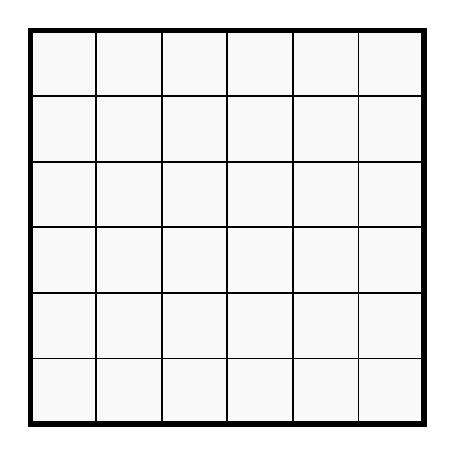
\begin{tikzpicture}[scale = 5.]
	\coordinate[](a) at (0,0);
	\coordinate[](b) at (1,0);	
	\coordinate[](c) at (1,1);
	\coordinate[](d) at (0,1);
	
	\pgfmathsetmacro{\h}{1}	
 	\pgfmathsetmacro{\dh}{1/6}
	
	% Trave
	\filldraw[fill=gray!5!white, line width=2pt, draw=black] 
	(a) -- (b) -- (c) -- (d) -- cycle;

	\begin{scope}[]
	\foreach \x in {1,2,...,5}
	{
	\draw[line width=0.7pt, draw=black] (\x*\dh,  0) -- (\x*\dh,\h);
	\draw[line width=0.7pt, draw=black] (0, \x*\dh) -- (\h, \x*\dh);
	}
	\end{scope}
		
\end{tikzpicture}
%\end{center}
%\caption{Square Problem (regular mesh)}
%\end{figure}
%
%\end{document}}
\hspace{5pt}
\subfigure[Trapezoidal mesh \label{fig:square_trapezoidal}]{%\documentclass{article}
%
%\usepackage{tikz}
%\usepackage{tikz-3dplot}
%\usetikzlibrary{calc}
%\usetikzlibrary{patterns}
%\usetikzlibrary{intersections}
%\usetikzlibrary{arrows}
%\tikzset{>=latex}
%
%\begin{document}
%
%\begin{figure}[!h]
%\begin{center}

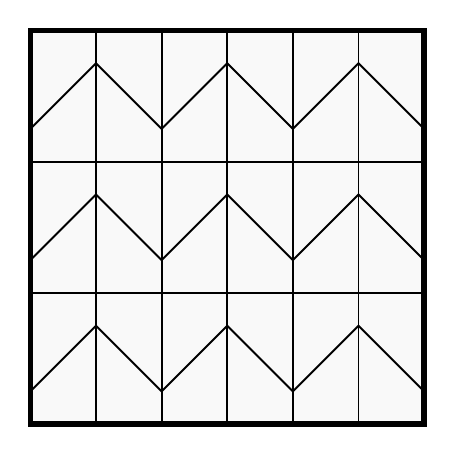
\begin{tikzpicture}[scale = 5.]
	\coordinate[](a) at (0,0);
	\coordinate[](b) at (1,0);	
	\coordinate[](c) at (1,1);
	\coordinate[](d) at (0,1);
	
	\pgfmathsetmacro{\h}{1}	
 	\pgfmathsetmacro{\dh}{1/6}
	
	% Trave
	\filldraw[fill=gray!5!white, line width=2pt, draw=black] 
	(a) -- (b) -- (c) -- (d) -- cycle;

	\begin{scope}[]
	\foreach \x in {1,3,...,5}
	{
	\draw[line width=0.7pt, draw=black] 
	(0, \x*\dh-\dh/2) -- (\dh, \x*\dh+\dh/2) -- (2*\dh, \x*\dh-\dh/2) -- 
	(3*\dh, \x*\dh+\dh/2) -- (4*\dh, \x*\dh-\dh/2) -- (5*\dh, \x*\dh+\dh/2)
	-- (6*\dh, \x*\dh-\dh/2);
	}
	\end{scope}
	
	\begin{scope}[]
	\foreach \x in {1,2,...,5}
	{
	\draw[line width=0.7pt, draw=black] (\x*\dh,  0) -- (\x*\dh,\h);
	}
	\end{scope}
	
	\begin{scope}[]
	\foreach \x in {2,4,...,5}
	{
	\draw[line width=0.7pt, draw=black] (0, \x*\dh) -- (\h, \x*\dh);
	}
	\end{scope}	
	
	
		
\end{tikzpicture}
%\end{center}
%\caption{Square Problem (irregular mesh)}
%\end{figure}
%
%\end{document}}
\caption{Square Problem}
\end{center}
\end{figure}
%
\begin{figure}[!ht]
\begin{center}
\subfigure[Regular mesh \label{fig:square_regular}]
{%\documentclass{article}
%
%\usepackage{graphicx}
%\usepackage{xcolor}
%\usepackage{colortbl}
%\usepackage{fp}
%\usepackage{tikz, pgfplots}
%\usetikzlibrary{calc}
%\usetikzlibrary{patterns}
%\usetikzlibrary{intersections}
%\usetikzlibrary{arrows}
%\tikzset{>=latex}
%
%% Color definition
%\definecolor{green2}{RGB}{154, 205, 50}
%\definecolor{green3}{RGB}{141, 182, 0}
%\definecolor{blue2}{RGB}{0, 102, 255}
%\definecolor{lightgreen}{RGB}{178,255,102}
%
%
%\begin{document}
%\scriptsize
%\begin{figure}[!h]
%\begin{center}
\begin{tikzpicture}
 %transpose legend
 \begin{loglogaxis}[width=0.45\textwidth, height=0.45\textwidth,
  legend style={anchor=south, at={(0.5, 1.07)}, draw=none, font=\scriptsize},
  grid=major,
  legend columns=3,
  xlabel={\large Number of Elements},
  ylabel={\Large $\frac{\parallel u_{h}-u \parallel_{L^{2}}}{\parallel u \parallel_{L^{2}}}$},
  xmin=1, xmax=1e5,
  ymin=1e-3, ymax=1e0,
  ytick={1e-3, 1e-2, 1e-1, 1},
  yticklabels={$10^{-3}$, $10^{-2}$, $10^{-1}$, $10^{0}$},
  xtick={1e0, 1e1, 1e2, 1e3, 1e4, 1e5},
  xticklabels={$10^{0}$, $10^{1}$, $10^{2}$, $10^{3}$, $10^{4}$, $10^{5}$},
 ]
 % Reference
 %\addplot[black, ultra thick] coordinates{
 %(50, 1.8248e-5)
 %(15000, 1.8248e-5)
 %}; 
 %\addlegendentry{Reference} 
 %
 \addplot[red, mark=+, thick, mark options={solid}]
 table [x index={0}, y index={1}]
 {figure/square/elastic_error_disp_u_peers_ver2.txt};
 \addlegendentry{PEERS \textbf{2B}}
 %
 \addplot[blue, mark=x, thick, mark options={solid}]
 table [x index={0}, y index={1}]
 {figure/square/elastic_error_disp_u_abf_ver2.txt};
 \addlegendentry{ABF \textbf{2B}}
 %
% \addplot[green3, mark=o, thick, mark options={solid}]
% table [x index={0}, y index={1}]
% {square_example/bolla1_type1/elastic_error_disp_u_l2_lmu3.txt};
% \addlegendentry{$\alpha / \mu=3$}
 %
 %\addplot[red, mark=+, dashed, very thick]
 %table [x index={0}, y index={1}]
 %{};
 %\addlegendentry{}
 %
 %\addplot[blue, mark=x, very thick]
 %table [x index={0}, y index={1}]
 %{};
 %\addlegendentry{}
 %
 %\addplot[green3, mark=x, very thick]
 %table [x index={0}, y index={1}]
 %{};
 %\addlegendentry{}
 % 
 \end{loglogaxis}
\end{tikzpicture}
%\end{center}
%\caption{The relative error versus the number of elements measured relative 
%to the $L^{2}$}
%\end{figure}
%
%\end{document}
}	
\subfigure[Trapezoidal mesh \label{fig:square_trapezoidal}]{%\documentclass{article}
%
%\usepackage{graphicx}
%\usepackage{xcolor}
%\usepackage{colortbl}
%\usepackage{fp}
%\usepackage{tikz, pgfplots}
%\usetikzlibrary{calc}
%\usetikzlibrary{patterns}
%\usetikzlibrary{intersections}
%\usetikzlibrary{arrows}
%\tikzset{>=latex}
%
%% Color definition
%\definecolor{green2}{RGB}{154, 205, 50}
%\definecolor{green3}{RGB}{141, 182, 0}
%\definecolor{blue2}{RGB}{0, 102, 255}
%\definecolor{lightgreen}{RGB}{178,255,102}
%
%
%\begin{document}
%\scriptsize
%\begin{figure}[!h]
%\begin{center}
\begin{tikzpicture}
 %transpose legend
 \begin{loglogaxis}[width=0.45\textwidth, height=0.45\textwidth,
  legend style={anchor=south, at={(0.5, 1.07)}, draw=none, font=\scriptsize},
  grid=major,
  legend columns=2,
  xlabel={\small Number of Elements},
  ylabel={\small $\parallel \bm{u}_{h}-\bm{u} \parallel_{L^{2}} / \parallel \bm{u} \parallel_{L^{2}}$},
  xmin=1, xmax=1e4,
  ymin=1e-4, ymax=1e0,
  ytick={1e-4, 1e-3, 1e-2, 1e-1, 1},
  yticklabels={$10^{-4}$, $10^{-3}$, $10^{-2}$, $10^{-1}$, $10^{0}$},
  xtick={1e0, 1e1, 1e2, 1e3, 1e4},
  xticklabels={$10^{0}$, $10^{1}$, $10^{2}$, $10^{3}$, $10^{4}$},
 ]
 % Reference
 %\addplot[black, ultra thick] coordinates{
 %(50, 1.8248e-5)
 %(15000, 1.8248e-5)
 %}; 
 %\addlegendentry{Reference} 
 \addplot[black, mark=square, thick, mark options={solid}]
 table [x index={0}, y index={1}]
 {figure/square/elastic_error_disp_u_peersq_trapezoidal.txt};
 \addlegendentry{PEERSQ} 
 %
 \addplot[green, mark=triangle, thick, mark options={solid}]
 table [x index={0}, y index={1}]
 {figure/square/elastic_error_disp_u_peers_trapezoidal_1b.txt};
 \addlegendentry{PEERSQ1B} 
 % 
 \addplot[red, mark=x, thick, mark options={solid}]
 table [x index={0}, y index={1}]
 {figure/square/elastic_error_disp_u_peers_trapezoidal_2b.txt};
 \addlegendentry{PEERSQ2B}
 %
 \addplot[red, mark=o, thick, mark options={solid}]
 table [x index={0}, y index={1}]
 {figure/square/elastic_error_disp_u_abf_trapezoidal_2b.txt};
 \addlegendentry{ABFQ2B}
 %
 \addplot[blue, mark=x, thick, mark options={solid}]
 table [x index={0}, y index={1}]
 {figure/square/elastic_error_disp_u_peers_trapezoidal_2bmixed.txt};
 \addlegendentry{PEERQ2BM }
 % 
 \addplot[blue, mark=o, thick, mark options={solid}]
 table [x index={0}, y index={1}]
 {figure/square/elastic_error_disp_u_abf_trapezoidal_2bmixed.txt};
 \addlegendentry{ABFQ2BM }
 %
% \addplot[green3, mark=o, thick, mark options={solid}]
% table [x index={0}, y index={1}]
% {square_example/bolla1_type1/elastic_error_disp_u_l2_lmu3.txt};
% \addlegendentry{$\alpha / \mu=3$}
 %
 %\addplot[red, mark=+, dashed, very thick]
 %table [x index={0}, y index={1}]
 %{};
 %\addlegendentry{}
 %
 %\addplot[blue, mark=x, very thick]
 %table [x index={0}, y index={1}]
 %{};
 %\addlegendentry{}
 %
 %\addplot[green3, mark=x, very thick]
 %table [x index={0}, y index={1}]
 %{};
 %\addlegendentry{}
 % 
 \end{loglogaxis}
\end{tikzpicture}
%\end{center}
%\caption{The relative error versus the number of elements measured relative 
%to the $L^{2}$}
%\end{figure}
%
%\end{document}
}
\caption{Error in $L^{2}$--norm of square problem}
\end{center}
\end{figure}

%\begin{figure}[!ht]
%\begin{center}
%%
%% Color definition
%\definecolor{green2}{RGB}{154, 205, 50}
%\definecolor{green3}{RGB}{141, 182, 0}
%\definecolor{blue2}{RGB}{0, 102, 255}
%\definecolor{lightgreen}{RGB}{178,255,102}
%
%
%\begin{document}
%\scriptsize
%\begin{figure}[!h]
%\begin{center}
\begin{tikzpicture}
 %transpose legend
 \begin{loglogaxis}[width=0.6\textwidth, height=0.6\textwidth,
  legend style={anchor=south, at={(0.5, 1.07)}, draw=none, font=\scriptsize},
  grid=major,
  legend columns=2,
  xlabel={\large Number of Elements},
  ylabel={\large $\parallel \bm{u}_{h}-\bm{u} \parallel_{L^{2}} / \parallel \bm{u} \parallel_{L^{2}}$},
  xmin=1, xmax=1e4,
  ymin=1e-2, ymax=1e2,
  ytick={1e-3, 1e-2, 1e-1, 1, 1e1},
  yticklabels={$10^{-3}$, $10^{-2}$, $10^{-1}$, $10^{0}$, $10^{1}$},
  xtick={1e0, 1e1, 1e2, 1e3, 1e4},
  xticklabels={$10^{0}$, $10^{1}$, $10^{2}$, $10^{3}$, $10^{4}$},
 ]
 % Reference
 %\addplot[black, ultra thick] coordinates{
 %(50, 1.8248e-5)
 %(15000, 1.8248e-5)
 %}; 
 %\addlegendentry{Reference} 
 %
 \addplot[red, mark=+, thick, mark options={solid}]
 table [x index={0}, y index={1}]
 {figure/square/elastic_error_disp_u_peers_ver2.txt};
 \addlegendentry{PEERS \textbf{2B}}
 %
 \addplot[blue, mark=x, thick, mark options={solid}]
 table [x index={0}, y index={1}]
 {figure/square/elastic_error_disp_u_abf_ver2.txt};
 \addlegendentry{ABF \textbf{2B}}
 %
 \addplot[red, mark=+, thick, dashed, mark options={solid}]
 table [x index={0}, y index={1}]
 {figure/square/elastic_error_disp_u_peers_trapezoidal_ver2.txt};
 \addlegendentry{PEERS \textbf{2B}}
 %
 \addplot[blue, mark=x, thick, dashed, mark options={solid}]
 table [x index={0}, y index={1}]
 {figure/square/elastic_error_disp_u_abf_trapezoidal_ver2.txt};
 \addlegendentry{ABF \textbf{2B}}
% \addplot[green3, mark=o, thick, mark options={solid}]
% table [x index={0}, y index={1}]
% {square_example/bolla1_type1/elastic_error_disp_u_l2_lmu3.txt};
% \addlegendentry{$\alpha / \mu=3$}
 %
 %\addplot[red, mark=+, dashed, very thick]
 %table [x index={0}, y index={1}]
 %{};
 %\addlegendentry{}
 %
 %\addplot[blue, mark=x, very thick]
 %table [x index={0}, y index={1}]
 %{};
 %\addlegendentry{}
 %
 %\addplot[green3, mark=x, very thick]
 %table [x index={0}, y index={1}]
 %{};
 %\addlegendentry{}
 % 
 \end{loglogaxis}
\end{tikzpicture}
%\end{center}
%\caption{The relative error versus the number of elements measured relative 
%to the $L^{2}$}
%\end{figure}
%
%\end{document}

%\caption{Error in $L^{2}$--norm of square problem}
%\end{center}
%\end{figure}



\subsection{Cantilever beam problem}
Now we consider the beam with length $L=10$ and height $l=2$ as we shown in Figure \ref{fig:beam}. The Young modulus is set equal to $E=1500$ and the Poisson $\nu=0.4999$.
The beam are fixed in the bottom left corner and subjected to a distributed load with $f=300$ on the right edge as shown in Figure \ref{fig:beam}.
\begin{figure}[!ht]
\begin{center}
%\documentclass{article}
%
%\usepackage{tikz}
%\usepackage{tikz-3dplot}
%\usetikzlibrary{calc}
%\usetikzlibrary{patterns}
%\usetikzlibrary{intersections}
%\usetikzlibrary{arrows}
%\tikzset{>=latex}
%
%\begin{document}
%
%\begin{figure}[!h]
%\begin{center}
\Large
\begin{tikzpicture}[scale = 1]
	
	\pgfmathsetmacro{\L}{10}	
 	\pgfmathsetmacro{\l}{2}	
	\pgfmathsetmacro{\dl}{2}
	
	
	\coordinate[](a) at (0,0);
	\coordinate[](b) at (\L,0);	
	\coordinate[](c) at (\L,\l);
	\coordinate[](d) at (0,\l);
	
	\coordinate[](m) at (0,\l/2);
	\coordinate[](mm) at (\L,\l/2);
	
	\coordinate[](t) at (\L+\dl,\l);
	\coordinate[](tt) at (\L+\dl-1,\l);
	\coordinate[](u) at (\L+\dl,0);
	\coordinate[](uu) at (\L+\dl+1,0);
	
	%% Quote
	\coordinate[](ql) at (0, -\dl/2);
	\coordinate[](qll) at (\L, -\dl/2);
	\coordinate[](qh) at (-\dl, 0);
	\coordinate[](qhh) at (-\dl, \l);
		

	% Trave
	\filldraw[fill=gray!10!white, line width=2pt, draw=black] 
	(a) -- (b) -- (c) -- (d) -- cycle;
	
	\begin{scope}[]
	\foreach \x in {1,2,...,4}
	{
	\draw[line width=0.7pt, draw=black] (\x*\dl,  0) -- (\x*\dl,\l);
	}
	\end{scope}	
	
	% Vincoli
	\begin{scope}[]
	\foreach \x in {0,1,...,2}
	{
	\filldraw[fill=black, line width=0.7pt, draw=black] 
	(-0.25,\l-\x*0.65) circle (0.25);
	}
	\end{scope}	
	
	\draw[line width=2pt, draw=black] 
	(a) -- (-0.5,0.3) -- (-0.5,-0.3) -- cycle;
	
	 %% Load
	\begin{scope}[->, ultra thick]
	\draw[->,line width=2.0pt,red] (t) -- (tt) node[red,midway,above]
	{$\textbf{-f}$};
	\draw[->,line width=2.0pt,red] (u) -- (uu) node[red,midway,below]
	{$\textbf{f}$};
	\draw[->,line width=2.0pt,red] (\L+\dl,3*\dl/4) -- (\L+\dl-0.5,3*\dl/4);
	\draw[->,line width=2.0pt,red] (\L+\dl,\dl/4) -- (\L+\dl+0.5,\dl/4);
	\end{scope}	
	\draw[line width=0.7pt, black, dashed] (t) -- (u) ;
	\draw[line width=0.7pt, black, dashed] (tt) -- (uu) ;	
	
	\draw[line width=0.7pt, black, dashdotted] (-1,1) -- (13,1) ;
	%% Quote
	\draw [<->,color=black] (ql) -- (qll) node[black,midway,above] {$L$};
	\draw [<->,color=black] (qh) -- (qhh) node[black,midway,left] {$l$};
	
	% Tratteggio
	\fill[pattern=north west lines, pattern color=black] 
	(-0.75,-0.4) rectangle (-0.5,\l+0.25);
	
	 %% Axis
	\begin{scope}[->, thick]
	\draw[->,line width=1.0pt,black] (0,\l+0.5) -- (0,\l+\dl);
	\draw[->,line width=1.0pt,black] (0,\l+0.5) -- (\l-0.5,\l+0.5);
	\end{scope}	
	\node[black,left] at (0,\l+\dl) {$\textbf{y}$};
	\node[black,above] at (\l-0.5,\l+0.5) {$\textbf{x}$};	
		
\end{tikzpicture}
%\end{center}
%\caption{Beam Cantilever}
%\end{figure}
%
%\end{document}
\caption{Cantilever Beam: Geometry problems \label{fig:beam}}
\end{center}
\end{figure}
We use to model the beam with two types of mesh: regular and trapezoidal as in the previous example (see Figures \ref{fig:square_regular} and \ref{fig:square_trapezoidal}).

\subsection{Cook's membrane}
The final example is the Cook's membrane. That is a typical benchmark and consist of a beam with vertex: $(0,0)$, $(48,44)$, $(48,60)$ and $(0,44)$.
The left vertical edge is clamped and the right vertical edge is subjected to the vertical distributed forces with resultant $F=100$ as shown in Figure \ref{fig:cook_membrane}.
The material properties are taken to be $E = 250$ and $\nu = 0.4999$, so that a nearly incompressible response is obtained.
We take into account the case of uniform meshes and the case of random distorted meshes (see Figure ).
\begin{figure}[!ht]
\begin{center}
%\documentclass{article}
%
%\usepackage{tikz}
%\usepackage{tikz-3dplot}
%\usetikzlibrary{calc}
%\usetikzlibrary{patterns}
%\usetikzlibrary{intersections}
%\usetikzlibrary{arrows}
%\tikzset{>=latex}
%
%\begin{document}
%
%\begin{figure}[!h]
%\begin{center}
\Large
\begin{tikzpicture}[scale = 0.1]
	\coordinate[](a) at (0,0);
	\coordinate[](b) at (48,44);	
	\coordinate[](c) at (48,60);
	\coordinate[](d) at (0,44);
	
	\coordinate[](Mu) at (50,44);
	\coordinate[](Muu) at (50,60);
	\coordinate[](Ml) at (50,52);
	
	\coordinate[](aa) at (0, 22);	
	\coordinate[](bb) at (48,52);
	\coordinate[](cc) at (24,22);
	\coordinate[](dd) at (24,52);
	
	\coordinate[](Ql) at (0,-5);	
	\coordinate[](Qll) at (48,-5);
	\coordinate[](Qh) at (-10,0);	
	\coordinate[](Qhh) at (-10,44);
	\coordinate[](Qhhh) at (-10,60);	
	
	% Trave
	\filldraw[fill=gray!10!white, line width=2pt, draw=black] (a) -- (b) -- (c) -- (d) -- cycle;
	\draw[line width=1pt, black] (aa) -- (bb);
	\draw[line width=1pt, black] (cc) -- (dd);
	
	% Tratteggio
	\fill[pattern=north west lines, pattern color=black] (d) rectangle (-3,0);
	
	 %% Load
	\begin{scope}[->, ultra thick]
	\draw[->,line width=2.0pt,red] (Mu) -- (Muu);
	\end{scope}	
	\node[red,right] at (Ml) {$\textbf{F}$};
		
	\fill[red] node at (c) {$\bullet$};	
	\node[red,above] at (c) {$\textbf{A}$};
	
	%% Quote
	\draw [<->,color=black] (Ql) -- (Qll) node[black,midway,above] {$48$};
	\draw [<->,color=black] (Qh) -- (Qhh) node[black,midway,left] {$44$};
	\draw [<->,color=black] (Qhh) -- (Qhhh) node[black,midway,left] {$16$};
			
\end{tikzpicture}
%\end{center}
%\caption{Cook's Membrane}
%\end{figure}
%
%\end{document}
\caption{Cook's Membrane Geometry \label{fig:cook_membrane}}
\end{center}
\end{figure}
We report in Figures \ref{fig:cook_reg_peers} and \ref{fig:cook_reg_abf}, the vertical displacement of the point $A$ versus the number of element per side for different PEERS and ABF elements in the case of regular mesh.
In the case of random distorted mesh the same results are shown in Figures  \ref{fig:cook_dist_peers} and \ref{fig:cook_dist_abf}.
It can be observe that the standard solution obtained  
%
\begin{figure}[!ht]
\begin{center}
\subfigure[Regular mesh \label{fig:cook_reg_peers}]{%\documentclass{article}

%\usepackage{graphicx}
%\usepackage{xcolor}
%\usepackage{colortbl}
%\usepackage{fp}
%\usepackage{tikz, pgfplots}
%\usetikzlibrary{calc}
%\usetikzlibrary{patterns}
%\usetikzlibrary{intersections}
%\usetikzlibrary{arrows}
%\tikzset{>=latex}
%
%% Color definition
%\definecolor{green2}{RGB}{154, 205, 50}
%\definecolor{green3}{RGB}{141, 182, 0}
%\definecolor{blue2}{RGB}{0, 102, 255}
%\definecolor{lightgreen}{RGB}{178,255,102}


%\begin{document}

%\begin{figure}[!h]
%\begin{center}
\begin{tikzpicture}
 %transpose legend
 \begin{axis}[width=0.45\textwidth, height=0.45\textwidth,
  legend style={anchor=south, at={(0.5, 1.07)}, draw=none, font=\scriptsize},
  legend columns=2,
  xlabel={\small Number of Elements per Side},
  ylabel={\small Vertical displacement of point A},
  xmin=0, xmax=66,
  ymin=10, ymax=16,
  ytick={5, 6, 7, 8, 9, 10, 11, 12, 13, 14, 15, 16},
  yticklabels={$5$, $6$, $7$, $8$, $9$, $10$, $11$, $12$, $13$, $14$, $15$, $16$},
  xtick={0, 4, 8, 16, 32, 64},
  xticklabels={$0$, $4$, $8$, $16$, $32$, $64$},
 ]
 % Reference
 %\addplot[black, ultra thick] coordinates{
 %(50, 1.8248e-5)
 %(15000, 1.8248e-5)
 %}; 
 %\addlegendentry{Reference} 
 %
 \addplot[black, mark=square, thick, mark options={solid}]
 table [x index={0}, y index={1}]
 {figure/cook/cook_regular_peersq.txt};
 \addlegendentry{PEERSQ} 
 %
 \addplot[green, mark=triangle, thick, mark options={solid}]
 table [x index={0}, y index={1}]
 {figure/cook/cook_regular_peers_1b_v1.txt};
 \addlegendentry{PEERSQ1B (v.1)}
 %
 \addplot[red, mark=o, thick, mark options={solid}]
 table [x index={0}, y index={1}]
 {figure/cook/cook_regular_peers_2b.txt};
 \addlegendentry{PEERSQ2B} 
 % 
 \addplot[blue, mark=x, thick, mark options={solid}]
 table [x index={0}, y index={1}]
 {figure/cook/cook_regular_peers_2bm.txt};
 \addlegendentry{PEERSQ2BM}


% %
% \addplot[green3, mark=o, thick, dashed, mark options={solid}]
% table [x index={0}, y index={1}]
% {figure/cook/cook_regular_peers_ver3_ver2.txt};
% \addlegendentry{PEERSQ1B (v.2)}
% % 

 \end{axis}
\end{tikzpicture}
%\end{center}
%\caption{Vertical Displacement of point A vs. the number of element per side}
%\end{figure}

%\end{document}}
%\subfigure[Random mesh \label{fig:cook_dist_peers}]{\input{figure/cook/cook_convergence_peers_random}}
\caption{Cook's Membrane (PEERSQ): Vertical Displacement of Point A vs. Element per Side}
\end{center}
\end{figure}
%
\begin{figure}[!ht]
\begin{center}
\subfigure[Regular mesh \label{fig:cook_reg_abf}]{\input{figure/cook/cook_convergence_abf}}
%\subfigure[Random mesh \label{fig:cook_dist_abf}]{%\documentclass{article}

%\usepackage{graphicx}
%\usepackage{xcolor}
%\usepackage{colortbl}
%\usepackage{fp}
%\usepackage{tikz, pgfplots}
%\usetikzlibrary{calc}
%\usetikzlibrary{patterns}
%\usetikzlibrary{intersections}
%\usetikzlibrary{arrows}
%\tikzset{>=latex}
%
%% Color definition
%\definecolor{green2}{RGB}{154, 205, 50}
%\definecolor{green3}{RGB}{141, 182, 0}
%\definecolor{blue2}{RGB}{0, 102, 255}
%\definecolor{lightgreen}{RGB}{178,255,102}


%\begin{document}

%\begin{figure}[!h]
%\begin{center}
\begin{tikzpicture}
 %transpose legend
 \begin{axis}[width=0.45\textwidth, height=0.45\textwidth,
  legend style={anchor=south, at={(0.5, 1.07)}, draw=none, font=\scriptsize},
  legend columns=2,
  xlabel={Number of Elements per Side},
  ylabel={Vertical displacement of point A},
  xmin=0, xmax=32,
  ymin=5, ymax=9,
  ytick={5, 6, 7, 8, 9},
  yticklabels={$5$, $6$, $7$, $8$, $9$},
  xtick={0, 2, 4, 8, 16, 32},
  xticklabels={$0$, $2$, $4$, $8$, $16$, $32$},
 ]
 % Reference
 %\addplot[black, ultra thick] coordinates{
 %(50, 1.8248e-5)
 %(15000, 1.8248e-5)
 %}; 
 %\addlegendentry{Reference} 
 %
 \addplot[red, mark=+, thick, mark options={solid}]
 table [x index={0}, y index={1}]
 {figure/cook/cook_random_abf_ver1.txt};
 \addlegendentry{ABF \textbf{2B} (mixed)}
 %
 \addplot[blue, mark=x, thick, mark options={solid}]
 table [x index={0}, y index={1}]
 {figure/cook/cook_random_abf_ver2.txt};
 \addlegendentry{ABF \textbf{2B}}
 %
 \addplot[green3, mark=o, thick, mark options={solid}]
 table [x index={0}, y index={1}]
 {figure/cook/cook_random_abf_ver3_ver1.txt};
 \addlegendentry{ABF \textbf{1B} (version 1)}
 %
 \addplot[green3, mark=o, thick, dashed, mark options={solid}]
 table [x index={0}, y index={1}]
 {figure/cook/cook_random_abf_ver3_ver2.txt};
 \addlegendentry{ABF \textbf{1B} (version 2)}
 % 
 \end{axis}
\end{tikzpicture}
%\end{center}
%\caption{Vertical Displacement of point A vs. the number of element per side}
%\end{figure}

%\end{document}}
\caption{Cook's Membrane (ABF): Vertical Displacement of Point A vs. Element per Side}
\end{center}
\end{figure}